\documentclass{article}
\usepackage{fullpage,fourier,amsmath,amssymb}
\usepackage{listings,color,url,hyperref}
\usepackage{epigraph, graphicx}
\usepackage[x11names]{xcolor}

\title{Assignment X \\ Bunco}
\author{Prof. Darrell Long \\
CSE 13S -- Winter 2020}
% \date{Due: October 13$^\text{th}$ at 11:59 pm}

\definecolor{codegreen}{rgb}{0,0.5,0}
\definecolor{codegray}{rgb}{0.5,0.5,0.5}
\definecolor{codepurple}{rgb}{0.58,0,0.82}

\lstloadlanguages{C,make,python,fortran}

\lstdefinestyle{c99}{
    morekeywords={bool, uint8_t, uint16_t, uint32_t, uint64_t, int8_t, int16_t, int32_t, int64_t},
    commentstyle=\color{codegreen},
    keywordstyle=\color{magenta},
    numberstyle=\tiny\color{codegray},
    identifierstyle=\color{blue},
    stringstyle=\color{codepurple},
    basicstyle=\ttfamily,
    breakatwhitespace=false,
    breaklines=true,
    captionpos=b,
    keepspaces=true,
    numbers=left,
    numbersep=5pt,
    showspaces=false,
    showstringspaces=false,
    showtabs=false,
    tabsize=4
}

\lstset{language=C, style=c99}

\begin{document}\maketitle

%%%%%%%%%%%%%%%%%%%%%%%%%%%%%%%%%%%%%%%%%%%%%%%%%%%%%%%%

\section{Introduction}
\epigraphwidth=0.5\textwidth
\epigraph{\emph{The gambling known as business looks with austere disfavor
upon the business known as gambling.}}{---Ambrose Bierce}

\noindent We are going to implement a simple game called \emph{Left, Right, and Center}.
It requires no skill, no real decision-making, and a player that is out of the
game can suddenly come back in and often win.

Some of you may have religious or moral prohibitions against gambling. This
program is not gambling, since (i) you neither win nor lose, and (ii) only
fictitious people lose or win any money. But, if you do have any qualms, let
us know and we will give you an alternative assignment.

\section{Playing the Game}
\epigraphwidth=0.75\textwidth
\epigraph{\emph{No sympathy for the devil; keep that in mind. Buy
the ticket, take the ride\ldots and if it occasionally gets a little
heavier than what you had in mind, well\ldots maybe chalk it off
to forced conscious expansion: Tune in, freak out, get beaten.}}{---Hunter
S. Thompson}

\begin{enumerate}
\item
Beginning with player $1$, roll the dice:
\begin{enumerate}
\item
If the player has \$3 or more then she rolls three dice;
if she has \$2 then she rolls two dice;
if she has only \$1 then she rolls one die;
if she has no money then she must pass.

\item For each die:
\begin{enumerate}
\item If the player rolls \textbf{L} then she gives \$1 to the player on her \emph{left}.

\item If the player rolls \textbf{R} then she gives \$1 to the player on her \emph{right}.

\item If the player rolls \textbf{C} then she puts \$1 in the pot in the
    \emph{center}.

\item If the player rolls \textbf{\textbullet} then she ignores it.
\end{enumerate}

\end{enumerate}
\item Move to the next player in sequence: to the
right. The players are numbered. There is \texttt{you}. Then there
is the left player which is (\texttt{you} $-$ 1) \texttt{mod} number
of players and there is the right player which is (\texttt{you} $+$
1) \texttt{mod} number of players.
\begin{lstlisting}
//
// Returns the position of the player to the left.
//
// pos:     The position of the current player.
// players: The number of players in the game.
//
uint32_t left(uint32_t pos, uint32_t players) {
  return ((pos + players - 1) % players);
}

//
// Returns the position of the player to the right.
//
// pos:     The position of the current player.
// players: The number of players in the game.
//
uint32_t left(uint32_t pos, uint32_t players) {
  return ((pos + 1) % players);
}
\end{lstlisting}

\item Repeat until only one player has any money remaining (who then wins the pot).
\end{enumerate}

%%%%%%%%%%%%%%%%%%%%%%%%%%%%%%%%%%%%%%%%%%%%%%%%%%%%%%%%

\section{Your Task}
\epigraphwidth=0.6\textwidth
\epigraph{
\emph{Any one who considers arithmetical methods of producing random digits
is, of course, in a state of sin.}}{---John von Neumann, 1951}

\begin{itemize}

\item You must have one source file: \texttt{bunco.c}. Do not name
your source file anything else. You will lose points.


\item For grading purposes the numbering of the faces matters, and
so they must be defined as follows (do not change it):

\begin{lstlisting}
typedef enum faciem {LEFT, RIGHT, CENTER, PASS} faces;
faces die[] = {LEFT, RIGHT, CENTER, PASS, PASS, PASS};
\end{lstlisting}

% \item You must give your players names, and for grading purposes the names
% must correspond to these (do not change them):

% {\small
% \begin{lstlisting}
% const char *names[] = {"Whoopi", "Dale",  "Rosie", "Jimmie", "Barbara",
%                        "Kyle",   "Raven", "Tony",  "Jenny",  "Clint"};
% \end{lstlisting}
% }

% \item Typing \texttt{make} must build your program and
% \texttt{./lrc} must run your program. Since you have not learned
% about \texttt{Makefiles} yet, here is one that you can use for now.

% \begin{lstlisting}[title=\texttt{Makefile}]
% CFLAGS=-Wall -Wextra -Werror -pedantic
% CC=clang $(CFLAGS)

% lrc     :       lrc.o
%         $(CC) -o lrc lrc.o
% lrc.o   :       lrc.c
%         $(CC) -c lrc.c
% clean   :
%         rm -f lrc lrc.o
% \end{lstlisting}

\item You will need to use a random number generator to simulate
rolling a dice. You can do this by calling the function \texttt{rand()}
(read the \emph{man page}) to get a random value. You can then use \texttt{mod}
to limit this value to the range of 0--5 inclusive (in computer science, we start from 0).
This value is used to determine what was rolled.

\item In order that your program be \emph{reproducible}, you must start from a
known place. This is accomplished by \emph{setting the random seed}
using the function \texttt{srand()} (again read the \emph{man page}).
Your program will ask for two numbers: the random seed and the
number of players. You should set these inputs to a variable to use
in your program. The random seed completely determines the outcome of your program. If you give it
the same random seed and the number of players you \emph{must} get
the same answer. Here is an example of using \texttt{srand()} and
\texttt{rand()}:
\begin{lstlisting}
srand(1); // This sets your random seed to 1.
int a = rand(); // Declares & initializes variable to random number.
\end{lstlisting}

\item \emph{Comment your code.} Include block comments to tell the grader what a certain block of code does. Use a line comment to explain something that is not as obvious. Refer to the coding standards.

\item Your program must use \texttt{clang-format}.

\item Your program \emph{must} run on the time share. If it does not, your program will receive a 0. To avoid this, test your program on the time share.

\item Your program must pass \texttt{infer} with no errors. If there are any, make sure to document them in your \texttt{README}.

\end{itemize}

% You should think carefully about what quantities that you must track
% in order for your program to function. At a \emph{minimum} you must
% keep track of the bank balance of each player, the amount of money
% in the pot, and the number of players that are \emph{in}. Be careful:
% players that were \emph{out} may be brought back in if money is
% passed to the \emph{left} or \emph{right}.

In lecture we talked briefly about \emph{random} and \emph{pseudo-random}
numbers. As we know, computers usually produce pseudo-random numbers, and in this case
it is to your benefit since \emph{reproducibility} is essential. That means
that in reality you program though it appears to be random is actually
\emph{deterministic}. This is why starting with the same seed produces the same sequence.

%%%%%%%%%%%%%%%%%%%%%%%%%%%%%%%%%%%%%%%%%%%%%%%%%%%%%%%%
\section{Hints}
\epigraph{\emph{It is no use trying to sum people up. One must follow hints,
not exactly what is said, nor yet entirely what is done.}}{---Virginia Woolf}

\begin{enumerate}

\item \emph{\textcolor{red}{Start Now!}} You can always finish early.

\item You may find it helpful to draw out and run through a game to get a feel
    for the rules. Doing so may make it easier to visualize the game and design
    your program.
\item The game itself should be an infinite loop, where the condition to break
    out of this loop is when there is one active player remaining.
\item You should think carefully about what quantities that you
must track in order for your program to function. At a \emph{minimum}
you must keep track of the bank balance of each player, the amount
of money in the pot, and the number of players that are \emph{in}.
Be careful: players that were \emph{out} may be brought back in if
money is passed to the \emph{left} or \emph{right}.

\end{enumerate}

%%%%%%%%%%%%%%%%%%%%%%%%%%%%%%%%%%%%%%%%%%%%%%%%%%%%%%%%

\section{Deliverables}
\epigraph{\emph{The design process is about designing and prototyping and
making. When you separate those, I think the final result
suffers.}}{---Jonathan Ive}

You will need to turn in:

\begin{enumerate}
\item \texttt{bunco.c}: The source file which is your program.

\item \texttt{Makefile}: This is a file that will allow the grader to type
    \texttt{make} to compile your program. Typing \texttt{make} with no
    arguments must build your program.
\begin{itemize}
\item \texttt{CFLAGS=-Wall -Wextra -Werror -Wpedantic} must be included.
\item \texttt{CC=clang} must be specified.
\item \texttt{make clean} must remove all files that are compiler generated.
\item \texttt{make} should build your program, as should \texttt{make all}.
\item Your program executable must be named \texttt{lrc}.
\end{itemize}

\item \texttt{README.md}: This must be in markdown.
This must describe how to use your program and \texttt{Makefile}.

\item \texttt{DESIGN.md}: This must be in markdown. The design document
should describe your design for your program with enough detail
that a sufficiently knowledgeable programmer would be able to
replicate your implementation. This does not mean copying your
entire program in verbatim. You should instead describe how your
program works with supporting pseudo-code. For this program, pay
extra attention to how you describe your logic flow/algorithm in
\textbf{C}.

\end{enumerate}

% All of these files must be in the directory \texttt{assignmentX}.

%%%%%%%%%%%%%%%%%%%%%%%%%%%%%%%%%%%%%%%%%%%%%%%%%%%%%%%%

% \section{Submission}
% \epigraphwidth=0.5\textwidth
% \epigraph{\emph{Better three hours too soon than a minute too
% late.}}{---William Shakespeare}

% You \emph{must} turn in your assignment with \texttt{git} in the following manner:

% \begin{enumerate}
% \item Add it!
% \begin{lstlisting}
% git add lrc.c Makefile README.md DESIGN.pdf
% \end{lstlisting}
% In order to turn in your program, you will first add the files to
% your repository using the \texttt{git add <filenames>} command. You
% will be submitting these files into the \texttt{assignment2}
% directory.

% \item Commit it!
% \begin{lstlisting}
% git commit -am "Your commit message here"
% \end{lstlisting}
% Changes to these files will be committed to the repository with
% \texttt{git commit}. The command should also include a commit message
% describing what changes are included in the commit. For your final and last commit for submission, your commit message should be ``final submission''

% \item Push it!
% \begin{lstlisting}
% git push
% \end{lstlisting}
% The committed changes are then synced up with the remote server
% using the \texttt{git push} command. You must be sure to push your
% changes to the remote server or else they will not be received by
% the graders.

% \textcolor{red}{Your assignment is turned in \emph{only} after you have pushed.
% If you forget to push, you have not turned in your assignment and you will get
% a \emph{zero}. ``I forgot to push'' is not a valid excuse. It is \emph{highly} recommended to commit and push your changes \emph{often}.}
% \end{enumerate}


%%%%%%%%%%%%%%%%%%%%%%%%%%%%%%%%%%%%%%%%%%%%%%%%%%%%%%%%%%%

% \newpage
% \section*{Example}
% \begin{verbatim}
% unix [109]% ./lrc
% Random seed: 1234
% How many players? 4
% Whoopi rolls... gives $1 to Jimmie gets a pass gets a pass
% Dale rolls... gets a pass gets a pass gets a pass
% Rosie rolls... gives $1 to Dale puts $1 in the pot puts $1 in the pot
% Jimmie rolls... gives $1 to Rosie gets a pass gets a pass
% Whoopi rolls... gets a pass gets a pass gives $1 to Jimmie
% Dale rolls... gets a pass puts $1 in the pot gives $1 to Whoopi
% Rosie rolls... gets a pass
% Jimmie rolls... gets a pass puts $1 in the pot puts $1 in the pot
% Whoopi rolls... puts $1 in the pot gives $1 to Jimmie
% Dale rolls... gives $1 to Whoopi gives $1 to Whoopi
% Rosie rolls... gets a pass gets a pass
% Jimmie rolls... gives $1 to Rosie puts $1 in the pot puts $1 in the pot
% Whoopi rolls... gives $1 to Jimmie
% Rosie rolls... gives $1 to Dale gets a pass puts $1 in the pot
% Jimmie rolls... gets a pass gives $1 to Rosie
% Rosie rolls... gets a pass gets a pass
% Jimmie rolls... gives $1 to Rosie
% Rosie wins the $9 pot with $3 left in the bank!

% \end{verbatim}

% \begin{figure}[ht]
%   \centering
%     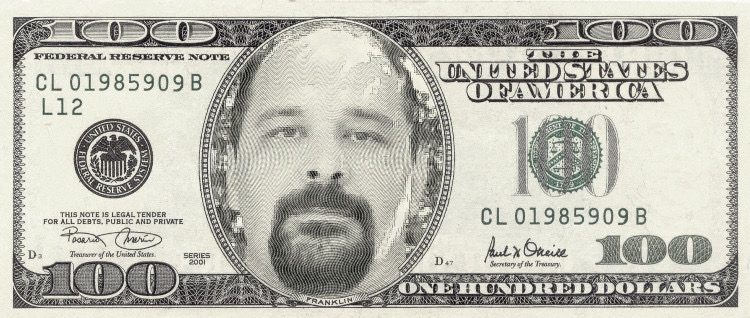
\includegraphics[width=5in]{darrelldollar.jpeg}
% \end{figure}
\end{document}
